\chapter{Einführung und Überblick}
% aus PP -> Worum geht es in dem projekt überhaupt?
%Keine detailierten Use cases, sondern kurz und knackig erläutern
Für die Entwicklung eines Multicast Test Tools mit unten stehenden Fähigkeiten
ist ein Zeitraum vom 21. Oktober 2010 bis 06. Mai 2011 veranschlagt worden.
Dieser Zeitraum beinhaltet sowohl die eigentliche Entwicklungszeit, als auch
Planungs- und Konzeptions- und Testphasen. Ebenfalls wurde für diese Phasen
ein Budget von 120.000€ veranschlagt.\\
\\
Eingesetzt werden soll das Multicast Test Tool für die Konfigurationsverifikation
eines Local-Area-Networks. Diese umfasst sowohl die Hardware- als auch die
Softwarekomponenten. Dadurch sollen Synchronität und Gleichlauf des gesamten
Netzwerkes überprüft und gegebenenfalls verbessert werden. Das Tool soll es ebenfalls ermöglichen, die Multicast-Fähigkeiten eines
Netzwerkes zu erfassen und zu validieren. Die Darstellung der Ergebnisse soll
möglichst übersichtlich und schnell erfassbar sein.\\
\\

Um diese Anforderungen zu erfüllen, wurden folgende Ziele definiert:\\
Es muss möglich sein mehrere (mindestens 30) Multicast Streams simultan
innerhalb eines Local-Area-Netzwerkes zu senden und zu empfangen. Zusätzlich
werden Statisiken für die Überprüfung benötigt. Hierfür werden Traversierungszeit,
Empfangsintervalle, sowie Anzahl der verlorengegangenen Pakete ermittelt und dem
Nutzer sichtbar gemacht.\\
\\
Um die Testbarkeit von verschiedenen Knotenpunkten innerhalb des Netzes zu
ermöglichen muss eine möglichst plattformunabhängige Lösung entwickelt werden. Hauptsächlich müssen Windows- 
sowie Linuxsysteme unterstüzt werden. \\
\\
Für eine möglichst übersichtliche und komfortable Benutzeroberfläche werden
Empfänger- und Senderprogramm zusammengefasst. 

%\chapter{Annahmen und Methoden}
%\section{Wichtigste Annahmen}
%by Dave
%ich denke das kann raus, "`Annahmen und Methoden"' reicht denke ich schon aus
%\section{Finanzkennzahlen}
% by Dave
% Finanzkennzahlen sind in etwa Return on Investment (ROI),
% Net present value oder Payback
% Ich bin dafür, dass wir den Punkt deshalb entfernen weil wir keine Anwendung
% finden. Grundlage ist nämlich immer ein investment(das wir nicht haben) :)
% by TobiScho
% ->Hört sich gut an
%\section{Kostenmodell}
%by Dave
%Kostenmodelle sind Ansätze auf verschiedener Basis, um den Aufwand (in
%Personenmonaten bzw. die Kosten (Finanziell) abzuschätzen, welcher notwendig ist, 
%um ein Produkt herzustellen.
%Uns bleit nur expertenbasierten Abschätzung/Bottom Up Methode -> hier kurz
% erläutern
\section{Nutzenargumentation}
%by Dave
%Welchen Nutzen hat das Projekt für den Kunden?
%Welchen Nutzen hat das Projekt für uns?
% -Profit
% -Längerfristige Geschäftsbeziehung
% -Spätere spezialisierung auf das Fachgebiet?
Das Multicast Test Tool bietet der Firma Net-Tools die Möglichkeit ihren Kunden ein
Tool für Multicast-Datenströme anzubieten. Tools andere Firmen sind an deren
Produkte gebunden. Durch den Vertrieb eines eigenen Tools kann die Firma
Net-Tools so bereits bestehende Kunden halten und neue gewinnen.\newline
\newline
Für die Firma SPAM bietet dieser Auftrag die Möglichkeit einen neuen Kunden zu
gewinnen und mit diesem eine langfristige Geschäftsbeziehung einzugehen. Die Entwicklung
des Tools soll exklusiv für die Firma Net-Tools geschehen, sodass ein Vertrieb
der Software an eventuelle Konkurrenten ausgeschlossen ist. Dies ist jedoch
vertretbar, da durch die langfristige Geschäftsbeziehung weitere Aufträge und
somit weiterer Profit für die Weiterentwicklung des Multicast Test Tools oder zur
Entwicklung anderer Tools erwartet wird.\newline
Eine eventuelle Spezialisierung auf den Bereich der Software für Netzwerktechnik
wäre als Gebiet zur Spezialisierung in Betracht zu ziehen, um aus dem dann
vorhandenen Skillset weitere Profite zu generieren.
%by TobiScho
%bitte mal drüber lesen und eventuell konstruktive kritik äußern
\section{Umfang und Abgrenzung}
%by Dave
%Was ist in scope, was ist out of scope?

\begin{itemize}
 \item[-]
 Das Multicast Test Tool soll dazu beitragen die Hardware und die Software
 eines Local-Area-Netzwerkes zu verifizieren um die Synchronität und den
 Gleichlauf des Netzwerkes zu verbessern.
  \item[-]
  Die Multicasting-Fähigkeiten einer Netzwerkinfrastruktur auf einen Blick erfass-
  und validierbar machen.
   \item[-]
   Das Tool soll plattformunabhängig sein, um den Blick auf das Netzwerk von
   verschiedenen Knoten aus zu ermöglichen.
    \item[-]
    Eine übersichtliche Oberfläche die sowohl Sender- als auch Empfängerprogramm
    zusammenfasst soll eine schnelle Einarbeitung und klare Bedienung ermöglichen.
     \item[-]
     Das Tool soll ausschließlich zum Testen einer Multicast Umgebung verwendet
     werden. Das Versenden von andersweitig relevanten Nutzdaten ist nicht vorgesehen.
      \item[-]
      Die Verwendung eines anderen Benutzerinterfaces als einer Java GUI oder eines 
      sehr einfachen Commandline Interface soll nicht ermöglicht werden.
       \item[-]
       Das Testen von anderen Protokollen neben Multicast für IP über Ethernet ist nicht vorgesehen.
       \end{itemize}

\chapter{Betriebswirtschaftliche Auswirkungen}
%\section{Finanzmodell}
%by Dave
%ich denke auch dieser Absatz ist für uns nicht von Nutzen
\section{Kostenabschätzung}

\subsection{Zugrunde liegende Personalkosten}

Folgende Kosten fallen für das entsprechende Personal an. Ein Manntag besteht
aus 8 Stunden.

\begin{table}[H]
\caption{Personalkosten nach Tätigkeitsbereich}
\label{tab:personal}
\begin{center}
\begin{tabular}{|l|c|r|}
\hline
\textbf{Jobtitel} & \textbf{Hauptgebiet} & \textbf{Kosten pro Stunde}\\
\hline
Projekt Manager & Organisation und Administration & 120 €\\
\hline
Produkt Manager & Analyse & 110 €\\
\hline
Leitender Ingenieur & Design & 100 €\\
\hline
Entwickler & Implementierung & 80 €\\
\hline
Systemtester & Systemtest & 80 €\\
\hline
Dokumentation & * & 70 € \\
\hline
\end{tabular}
\end{center}
\label{default}
\end{table}

\begin{figure}[H]
\centering
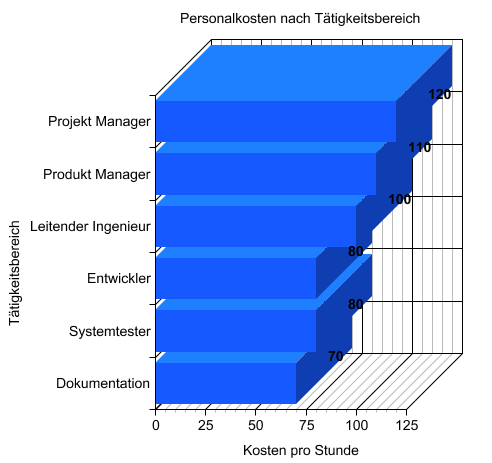
\includegraphics[width=10cm]{images/graph.png}
\label{img:perso}
\caption{Personalkosten nach Tätigkeitsbereich}
\end{figure}


\subsection{Kosten der Analysephase}

Für die Analysephase werden insgesamt 15 Manntage benötigt. Administration
und Organisation sind nicht eingerechnet. Die Kosten setzten sich aus folgenden
Komponenten zusammen.

\begin{table}[H]
\caption{Analyse - Personalkosten nach Tätigkeitsbereich}
\label{tab:kpersonal}
\begin{center}
\begin{tabular}{|l|r|r|}
\hline
\textbf{Jobtitel} & \textbf{Beteiligung} & \textbf{Kosten}\\
\hline
Produkt Manager & 50 \% & 6600 €\\ %0.5*15*110*8
\hline
Leitender Ingenieur & 30 \% & 3600 €\\ %0.3*15*100*8
\hline
Entwickler & 0 \% & 0 €\\ %0.0*15*80*8
\hline
Systemtester & 0 \% & 0 €\\ %0.0*15*80*8
\hline
Dokumentation & 20 \% & 1680 €\\ %0.2*15*70*8
\hline
\textbf{Gesamt} & \textbf{100 \%} & \textbf{11880 €}\\ %6600+3600+1680
\hline
\end{tabular}
\end{center}
\label{default}
\end{table}


\subsection{Kosten der Designphase}

Für die Designphase werden insgesamt 22 Manntage benötigt. Administration
und Organisation sind nicht eingerechnet. Die Kosten setzten sich aus folgenden
Komponenten zusammen.

\begin{table}[H]
\caption{Design - Personalkosten nach Tätigkeitsbereich}
\label{tab:kdesign}
\begin{center}
\begin{tabular}{|l|r|r|}
\hline
\textbf{Jobtitel} & \textbf{Beteiligung} & \textbf{Kosten}\\
\hline
Produkt Manager & 30 \% & 5808 €\\ %0.3*22*110*8
\hline
Leitender Ingenieur & 50 \% & 8800 €\\ %0.5*22*100*8
\hline
Entwickler & 0 \% & 0 €\\ %0.0*22*80*8
\hline
Systemtester & 0 \% & 0 €\\ %0.0*22*80*8
\hline
Dokumentation & 20 \% & 2464 €\\ %0.2*22*70*8
\hline
\textbf{Gesamt} & \textbf{100 \%} & \textbf{14854 €}\\%5808+8800+2464
\hline
\end{tabular}
\end{center}
\label{default}
\end{table}

\subsection{Kosten der Implementierungsphase}

Für die Implementierungsphase werden insgesamt 59 Manntage benötigt.
Administration und Organisation sind nicht eingerechnet. Diese Schätzung wurde
per Bottom-Up für die einzelnen Anforderungen berechnet. In dieser Zeit ist
bereits der Modultest enthalten.

\begin{table}[H]
\caption{Implementierung - Übersicht der Dauer per Anforderung}
\label{tab:kint}
\begin{center}
\begin{tabular}{|l|r|r|}
\hline
\textbf{Identifikator} & \textbf{Kurzbeschreibung} & \textbf{Personentage}\\
\hline
\textbf{/VA0100/} & Multicast-Sendefähigkeit & \textbf{2}\\
\hline
\textbf{/VA0200/} & Multicast-Empfangsfähigkeit & \textbf{2}\\
\hline
\textbf{/VA0300/} & Datenauswertung & \textbf{3}\\
\hline
\textbf{/VA0400/} & Gleichzeitigkeit & \textbf{2}\\
\hline
\textbf{/VA0500/} & Kompatibilität & \textbf{3}\\
\hline
\textbf{/VA0600/} & Konfigurierbarkeit & \textbf{2}\\
\hline
\textbf{/VA0700/} & Sendestatistik & \textbf{1}\\
\hline
\textbf{/VA0800/} & Konfigurationsdatei & \textbf{3}\\
\hline
\textbf{/VA0900/} & Grafische Nutzeroberfläche & \textbf{14}\\
\hline
\textbf{/VA1200/} & Messwertanzeige & \textbf{3}\\
\hline
\textbf{/VA1200/} & Textbasierte Nutzeroberfläche & \textbf{14}\\
\hline
\textbf{Gesamt} & \textbf{100 \%} & \textbf{49}\\
\hline
+ Puffer & 20 \% von 49 & 10\\
\hline
\textbf{Gesamt} & \textbf{100 \%} & \textbf{59}\\
\hline
\end{tabular}
\end{center}
\label{default}
\end{table}

Diese Kosten teilen sich folgendermaßen auf das Projektteam auf:

\begin{table}[H]
\caption{Implementierung - Personalkosten nach Tätigkeitsbereich}
\label{tab:kimp}
\begin{center}
\begin{tabular}{|l|r|r|}
\hline
\textbf{Jobtitel} & \textbf{Beteiligung} & \textbf{Kosten}\\
\hline
Produkt Manager & 5 \% & 2596 € \\ %0.05*59*110*8
\hline
Leitender Ingenieur & 15 \% & 7080 € \\ %0.15*59*100*8
\hline
Entwickler & 35 \% & 13216 € \\ %0.35*59*80*8
\hline
Systemtester & 30 \% & 11328 €\\ %0.30*59*80*8
\hline
Dokumentation & 15 \% & 4956 €\\ %0.15*59*70*8
\hline
\textbf{Gesamt} & \textbf{100 \%} & \textbf{39176
€}\\%2596+7080+13216+11328+4956
\hline
\end{tabular}
\end{center}
\label{default}
\end{table}


\subsection{Kosten der Integration- und Systemtestphase}

Für die Integration- und Systemtestphase werden insgesamt 40 Manntage benötigt.
Administration und Organisation sind nicht eingerechnet. Die Kosten setzten sich aus folgenden
Komponenten zusammen.

\begin{table}[H]
\caption{Integration und Systemtest - Personalkosten nach Tätigkeitsbereich}
\label{tab:kint}
\begin{center}
\begin{tabular}{|l|r|r|}
\hline
\textbf{Jobtitel} & \textbf{Beteiligung} & \textbf{Kosten}\\
\hline
Produkt Manager & 5 \% & 1760 €\\ %0.05*40*110*8
\hline
Leitender Ingenieur & 15 \% & 4800 €\\ %0.15*40*100*8
\hline
Entwickler & 30 \% & 7680 €\\ %0.30*40*80*8
\hline
Systemtester & 35 \% & 8960 €\\ %0.35*40*80*8
\hline
Dokumentation & 15 \% & 3360 €\\ %0.15*40*70*8
\hline
\textbf{Gesamt} & \textbf{100 \%} & \textbf{26560 €}\\%1760+4800+7680+8960+3360
\hline
\end{tabular}
\end{center}
\label{default}
\end{table}

\subsection{Kosten der Betriebs- und Wartungsphase}

Kosten für die Betriebs- und Wartungsphase werden nicht berücksichtigt, da
dieser Service nicht angeboten wird und vom Kunde nicht gefordert wurde.

\subsection{Kosten der Organisation und Administration}

Für Organisation und Administration durch den Projekt Manager wird pauschal eine
Stunde pro Werktag berechnet. Der Projekt Manager kommt ab dem 21. September
2010 bis zum 06. Mai 2011 zum Einsatz. In dieser Zeit befinden sich 164
Werktage(Mo-Fr inklusive Feiertage).\\
Bei einem Stundenlohn von 120 € betragen die Gesamtkosten 19680 €.%120*164

\subsection{Zusammenfassung}

\begin{table}[H]
\caption{Personalkosten des Projekts}
\label{tab:ktotal}
\begin{center}
\begin{tabular}{|l|r|}
\hline
\textbf{Beschreibung} & \textbf{Kosten}\\
\hline
Analyse & 11880 €\\
\hline
Design & 14854 €\\
\hline
Implementierung & 39176 €\\
\hline
Integration und Systemtest & 26560 €\\
\hline
Organisation und Administration & 19680 €\\
\hline
\textbf{Gesamt} & \textbf{112150 €} \\ %11880+14854+39176+26560+19680
\hline
\end{tabular}
\end{center}
\label{default}
\end{table}

Hinzu kommen Risikokosten, sowie eigenes Interesse. Der Abnahmepreis beläuft
sich daher auf 125000€.

\begin{figure}[H]
\centering
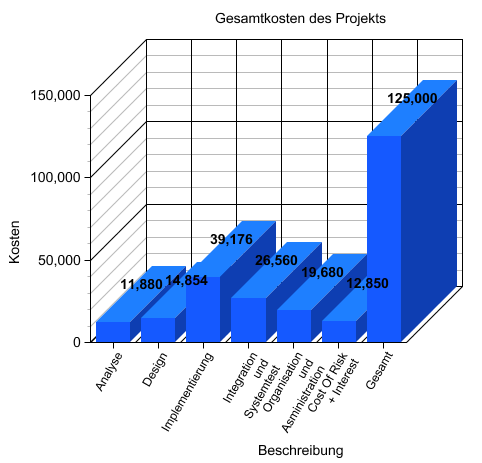
\includegraphics[width=10cm]{images/graph2.png}
\label{img:kost}
\caption{Kosten des Projekts}
\end{figure}

\section{Ergebnisanalyse}

Die geschätzten Gesamtkosten des Projekts betragen 112150 € und liegen damit im
gegebenen Budget.\\ Ob das Projekt rentabel sein wird kann erst nach den
Vertragsverhandlungen gesagt werden. Es bleibt abzuwarten, wieviel der Kunde
bereit ist zu zahlen. Nach den Verhandlungen kann näheres dazu gesagt
werden.\newline Sollte das Projekt nicht rentabel sein gibt es dennoch einen
guten Grund das Projekt zu starten. Die Tatsache, dass der Kunde an
einer Folgeversion interessiert ist und somit auf eine längere Geschäftsbeziehung wert legt, würde Anreiz zum Starten des Projekts bieten.

\chapter{Risiko- und Sensitivitätsanalyse}
\label{cha:risi}

\section{Produkt Risiken}
\label{sec:prorisk}

\paragraph{/R0100/}Hardwareausfälle \\
\texttt{Beschreibung:} Da Multicasting von vielen Netzwerkkomponenten nicht richtig unterstützt wird, könnte der Einsatz des Tools zu Hardwareausfällen führen.\\
\texttt{Wahrscheinlichkeit:} mittel\\
\texttt{Entdeckbarkeit:} hoch\\
\texttt{Schaden:} mittel\\
\texttt{Vermeidung:} Nicht möglich.\\
\texttt{Reaktion:} Austausch der Hardware.\\

\paragraph{/R0200/}Netzwerküberlastung\\
\texttt{Beschreibung:} Die Verwendung des Tools von ungeschulten Benutzern kann, wegen der Beschaffenheit von Multicast Protokollen, zu einer Netzüberlastung führen. \\
\texttt{Wahrscheinlichkeit:} mittel\\
\texttt{Entdeckbarkeit:} hoch\\
\texttt{Schaden:} gering\\
\texttt{Vermeidung:} Gute Dokumentation und Schulung der Benutzer.\\
\texttt{Reaktion:} Abschalten des Tools.\\

\section{Marktrisiken}
\label{sec:marketrisk}

\paragraph{/R1000/}Mitbewerber\\ 
\texttt{Beschreibung:} Der Fakt dass es vier direkte Mitbewerber gibt, die ein
Produkt für die exakt gleiche Zielgruppe entwickeln, könnte zum Untergang des
Produktes im Markt führen. \\ \texttt{Wahrscheinlichkeit:} mittel\\ \texttt{Entdeckbarkeit:} gering\\
\texttt{Schaden:} hoch\\
\texttt{Vermeidung:} Hohe Qualität des Tools.\\
\texttt{Reaktion:} Anpassen des Tools für Nischenbereiche.\\

\paragraph{/R1100/}Fähigkeiten der Entwickler\\
\texttt{Beschreibung:} Da das Team noch sehr wenig Praktische Erfahrung mit
Softwareprojekten sammeln konnte, sind starke Abweichungen bei dem geplanten
Zeitaufwand bis zur Fertigstellung, den benötigten Resourcen und der Qualität des Endproduktes sehr warrscheinlich. \\ 
\texttt{Wahrscheinlichkeit:} mittel\\ 
\texttt{Entdeckbarkeit:} mittel\\
\texttt{Schaden:} mittel\\
\texttt{Vermeidung:} Experten um Rat fragen, erhöhte Sorgfalt bei der Planung.\\
\texttt{Reaktion:} Reevaluierung der Schätzungen.\\
 
 \section{Entwicklungsrisiken}
 \label{sec:devrisk}

 \paragraph{/R2000/}Echtzeitfähigkeit\\
 \texttt{Beschreibung:} Java könnte durch seine Hardwareabstraktion und
 Speicherbereinigung die hohen Anforderungen an Echtzeitfähigkeit verfehlen. \\ \texttt{Wahrscheinlichkeit:} gering\\
 \texttt{Entdeckbarkeit:} hoch\\
 \texttt{Schaden:} mittel\\
 \texttt{Vermeidung:} Testcases entwickeln. \\
 \texttt{Reaktion:} Wechsel der Programmiersprache.\\

 \paragraph{/R2100/}Plattform Abstraktion\\
 \texttt{Beschreibung:} Durch Javas hohe Plattformabstraktion könnten Zugriffe
 auf niedriger Ebene, um zum Beispiel die Netzwerkkarte anzusprechen, nicht
 erlaubt sein. \\ \texttt{Wahrscheinlichkeit:} gering\\ \texttt{Entdeckbarkeit:} hoch\\
 \texttt{Schaden:} mittel\\
 \texttt{Vermeidung:} Testcases entwickeln.\\
 \texttt{Reaktion:} Schreiben der benötigten Komponenten in einer anderen Sprache.\\

\chapter{Fazit und Zusammenfassung}
%by Dave
%aufgreifen der Ergebnisanalyse und endgültige Entscheidung ob das projekt
% gestartet wird?
\paragraph{}Ausgehend von einer Bottom-Up-Analyse, die auf dem Zeitaufwand,
sowie den Personalkosten, für die einzelnen Entwicklungsphasen beruht, lässt sich der
finanzielle Aufwand für die Realisierung des Projektes auf ca. 112150 €
schätzen. \paragraph{}Für die Firma Net-Tools stellt die Software insofern einen
erheblichen Mehrwert dar, weil es bislang keine direkt vergleichbare Software
frei am Markt verfügbar gibt. Die Firma Net-Tools wird damit zum Branchenvorreiter im
Multicasting-Bereich. Im Hinblick auf Live-Video-Streaming und Internetfernsehen
hält dieser Bereich vielversprechende Wachstumsmöglichkeiten bereit.

\paragraph{}Unter Berücksichtigung dieses Mehrwerts hält die Firma SPAM
Software Programming And More einen Abnahmepreis von 125000 € für realisitisch.
Dieser Preis deckt auch die zu erwartenden Risiken ab.
\paragraph{}Von Seiten der Firma SPAM Software Programming And More wird das
Projekt sowohl technisch, als auch wirtschaftlich als umsetzbar angesehen und mit Zustimmung
der Firma Net-Tools wird das Projekt zur Umsetzung freigegeben.
